\scanpage{20}
\mspage{8}
Il revient au $=$ de dire que $\sigma_0,\sigma_1,\sigma_\infty,\rho$ sont des générateurs, avec relations de définition
\[
(4)\qquad
(\overbrace{\rho^{-1}\sigma_\infty\sigma_0\deleted{\rho}}^{l_\infty})
(\overbrace{\rho^{-1}\sigma_1\sigma_\infty\deleted{\rho}}^{l_1})
(\overbrace{\rho^{-1}\sigma_0\sigma_1\deleted{\rho}}^{l_0})=1
\]
\[
(5)\qquad \sigma_0^2=\sigma_1^2=\sigma_\infty^2=1
\]
\[
(6)\qquad \rho^3=1
\]
\margin{Il faut ajouter les relations $\rho\sigma_0\rho^{-1}=\sigma_1$ etc
On a deux gén. $\sigma_0,\rho$ en fait avec relations
\[
\sigma_0^2=\rho^3=1,
\]
la
\deleted{$\unsure{[\underset{\sigma_\infty}{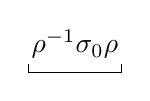
\begin{tikzpicture}[baseline=(term.base)]\node[inner sep=1pt] (term) {$\rho^{-1}\sigma_0\rho$};\draw ([yshift=-1pt]term.south west) -- ++(0,-3pt) -| ([yshift=-1pt]term.south east);\end{tikzpicture}}\sigma_0\rho^{-1}][\underset{\sigma_1}{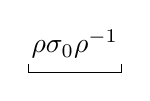
\begin{tikzpicture}[baseline=(term.base)]\node[inner sep=1pt] (term) {$\rho\sigma_0\rho^{-1}$};\draw ([yshift=-1pt]term.south west) -- ++(0,-3pt) -| ([yshift=-1pt]term.south east);\end{tikzpicture}}\underset{\sigma_\infty}{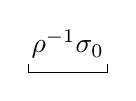
\begin{tikzpicture}[baseline=(term.base)]\node[inner sep=1pt] (term) {$\rho^{-1}\sigma_0$};\draw ([yshift=-1pt]term.south west) -- ++(0,-3pt) -| ([yshift=-1pt]term.south east);\end{tikzpicture}}\rho^{-1}]|[\underset{\sigma_\infty}{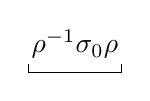
\begin{tikzpicture}[baseline=(term.base)]\node[inner sep=1pt] (term) {$\rho^{-1}\sigma_0\rho$};\draw ([yshift=-1pt]term.south west) -- ++(0,-3pt) -| ([yshift=-1pt]term.south east);\end{tikzpicture}}\sigma_0\rho^{-1}][\underset{\sigma_1}{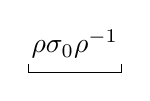
\begin{tikzpicture}[baseline=(term.base)]\node[inner sep=1pt] (term) {$\rho\sigma_0\rho^{-1}$};\draw ([yshift=-1pt]term.south west) -- ++(0,-3pt) -| ([yshift=-1pt]term.south east);\end{tikzpicture}}\underset{\sigma_\infty}{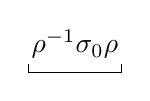
\begin{tikzpicture}[baseline=(term.base)]\node[inner sep=1pt] (term) {$\rho^{-1}\sigma_0\rho$};\draw ([yshift=-1pt]term.south west) -- ++(0,-3pt) -| ([yshift=-1pt]term.south east);\end{tikzpicture}}\rho^{-1}]}$}
relation (4) est conséquence des précédentes (vient du fait $\sigma_1=\rho\sigma_0\rho^{-1}$, \deleted{\illegible{1}} $\sigma_\infty=\rho^{-1}\sigma_0\rho$). Noter que
\[
\begin{aligned}
l_0&=\deleted{\unsure{(\rho\sigma_0\rho^{-1})^2|(\sigma_0\rho)^2}}\rho^{-1}(\sigma_0\rho)^2\rho
=\boxed{\rho^{-1}\sigma_0\rho\sigma_0\rho^{-1}}\\
l_1&=(\deleted{\unsure{\rho}}\sigma_0\rho)^2\\
l_\infty&=(\unsure{\rho^{\deleted{-1}}|\rho^{-1}}\sigma_0\deleted{\unsure{\rho}})^2
\end{aligned}
\]
\[
\begin{aligned}
\operatorname{int}(\sigma_0)l_1&=l_\infty\\
\operatorname{int}(\sigma_0)l_\infty&=l_1\\
\operatorname{int}(\sigma_0)(l_0)&=l_\infty^{-1}l_1^{-1}
\end{aligned}
\]}
\margin{\uline{NB}
\[
\begin{aligned}
\sigma_0(l_0)&=l_\infty^{-1}l_1^{-1}\\
\sigma_0(l_1)&=l_\infty\\
\sigma_0(l_\infty)&=l_1^{\deleted{\unsure{-1}}}\deleted{\unsure{l_\infty^{-1}|l_0^{-1}}}
\end{aligned}
\]
et itou pour $\sigma_1,\sigma_\infty$}
\uline{NB} Si on y fait \inserted{de plus} $\sigma_0,\sigma_1,\sigma_\infty=1$, on trouve comme relation de définition $\rho^3=1$, \deleted{\unsure{donc}} sans plus, ce qui prouve que $\rho$ n'est pas un mot \unsure{p.v.|p.r.} aux $\sigma_i$\ldots

Tout ceci est compatible avec les relations des débuts, \deleted{\unsure{si dans ces dernières on avait tout pris des primes}, et \unsure{qu'on interprète} $l_i'=l_i^{-1}$, $\sigma_i'=\sigma_{\unsure{\dot\rho(i)}}$}
\deleted{i.e. $\sigma_i$} \deleted{\unsure{de notre groupe|de sorte que} $\unsure{\mathcal E'|\sigma_i'|\sigma'}$} si on y remplace les $l_i$ par les $l_i^{-1}$
Ici on a, comme $\sigma_i=\sigma^{\unsure{\prime|1}}_{\dot\rho^{-1}(i)}$
\[
(7)\quad\left\{\begin{aligned}
\operatorname{int}(\sigma_i)&:\text{ échange }l_j\text{ et }l_{\deleted{\unsure{j}}k}
\quad\inserted{(i,j,\unsure{k|h})\text{ distincts})}\ \deleted{\text{et}}\\[-2pt]
&\deleted{\text{(et le }\unsure{\text{dernier}|\text{devenir}}\ l_{\dot\rho(i)}\ \text{s'en déduit par (1))}}\\
\operatorname{int}(\rho)l_i&=l_{\dot\rho(i)}
\end{aligned}\right.
\]

On voudrait maintenant expliciter les $\varepsilon_i$ avec $\varepsilon_i^2=l_i$ $(i=0,1,\infty)$, $\varepsilon_i$ étant \unsure{donc un|un des} \unsure{générateurs|générateur} \unsure{du|des} centralisateur (ou normalisateur, c'est idem) des $L_i$ dans $\mathcal E^+$\unsure{.|,} (ou le centralisateur dans $\mathcal E$). Les calculs faits plus haut, avec les chgts de \unsure{notation|notations} indiqués, donnent
\[
\deleted{(8)}\quad\left\{\begin{aligned}
\unsure{\deleted{\varepsilon_0}|\varepsilon_0}&=l_0^{\deleted{\unsure{-1|4}}}\sigma_1 l_{\unsure{0|1}}^{\deleted{\unsure{-1|4}}}\\
\unsure{\deleted{\varepsilon_1}|\varepsilon_1}&=\unsure{\deleted{l_\infty^{-1}}|l_\infty^{-1}}\sigma_\infty \deleted{l_1^{-1}}\ \inserted{l_1}\\
\varepsilon_\infty&=l_0^{-1}\sigma_0 l_\infty
\end{aligned}\right.
\]
\mspage{19}
